\documentclass[a4paper,10pt]{article}
\include{amsymb}
\include{marvosym}

\usepackage[francais]{babel}
\usepackage[cyr]{aeguill}
\usepackage[applemac]{inputenc}
\usepackage{graphicx}
\usepackage{xspace}
\usepackage[a4paper]{geometry}
\usepackage{latexsym,amsmath,amssymb,textcomp}
\usepackage{moreverb}
\usepackage{listings}
\usepackage{multirow}
\usepackage{titling}
\usepackage{mathabx}

\usepackage{pdfpages}

\usepackage{hyperref}


\newlength{\indentationnota}
\newlength{\largeurlignenota}
\newlength{\paddingnota}
\newlength{\largeurnota}
\setlength{\paddingnota}{5pt}
\setlength{\largeurnota}{0.9cm}

\definecolor{pink}{rgb}{1,0.5,1}
\makeatletter

\newenvironment{pictonote}[1]{% on passe le nom du �chier en argument
\begin{list}{}{%
\setlength{\labelsep}{0pt}%
\setlength{\rightmargin}{15pt}%
\setlength{\paddingnota}{5pt}}
\item%
\setlength{\indentationnota}{%
\@totalleftmargin+\largeurnota+\paddingnota}%
\setlength{\largeurlignenota}{%
\linewidth-\largeurnota-\paddingnota}%
\parshape=3%
\indentationnota\largeurlignenota%
\indentationnota\largeurlignenota%
\@totalleftmargin\linewidth%
\raisebox{-\largeurnota+2.2ex}[0pt][0pt]{%
\makebox[0pt][r]{%
\includegraphics[width=\largeurnota]{#1}%
\hspace{\paddingnota}}}%
\ignorespaces}{%
\end{list}}

\makeatother

\newenvironment{attention}%
{\begin{pictonote}{/Users/benjamin/Documents/Education/LaTeX/danger}}%
{\end{pictonote}}

\newenvironment{unicorn}%
{\begin{pictonote}{/Users/benjamin/Documents/Education/LaTeX/angry_unicorn}}%
{\end{pictonote}}

\newcommand\unicornbox[1]{\colorbox{pink}{\color{white}{#1}}}

\newcommand\cf{\emph{c.f}}

\newcommand\signature{%
\begin{figure}[br]
	\begin{flushright}
	\begin{minipage}{8cm}
		\begin{center}
		\reflectbox{\includegraphics[width=8cm]{/Users/benjamin/Documents/Education/LaTeX/unicorn}}\\
		\theauthor
		\end{center}
	\end{minipage}
	\end{flushright}
\end{figure}}

\newcommand\danger{\raisebox{-0.4ex}{\LARGE $\triangle$ \normalsize} \hspace{-4.1ex}! \hspace{1ex}}
\newcommand\PL{Programmation Logique\xspace}
\newcommand\pl{\bsc{Prolog}\xspace}


\title{Multi touch support implementation in Pharo}
\author{Fran�ois \bsc{Lepan}\\Benjamin \bsc{Van Ryseghem}}

\begin{document}
\maketitle

\vfill
\section*{Introduction}
During our project our main goal was to introduce a new way to handle multi touch events and gestures in Pharo.
Starting from what we previously did last semester during the PJE lecture and using the same approach, we introduce a handling of gestures based on TUIO with an architecture allowing to switch to virtual machine events.

In order to analyse these gestures we needed a state machine that would fill the gap between the human gesture
and a perfect gesture. This state machine has been improved as we were adding new gestures to fit as much as possible the gestures performed by the user.

Another goal was to clean and reunify the whole hierarchy of system events and to provide a clean abstraction
of low level data structure.

\vfill
\vfill
\newpage
\tableofcontents
\newpage

\section{TUOI and blobs analysis}
	
Our first goal is to be able to retrieve gestures from the user. In order to do we used TUIO which is a protocol for 
multitouch events. It retrieves the multi-touch gestures from the hardware and then generates events for each 
finger on the device (\emph{cf}~Fig.~\ref{fig:TUIO_platform_diagram}). For our tests we used a software called 
Tongseng \footnote{Fajran Iman Rusadi -  https://github.com/fajran/tongseng} that generates TUIO events from the Mac trackpad and a library created by Simon Holland\footnote{http://mcl.open.ac.uk/sh/squeakmusic.html} that parses the TUIO events.

\section{System events hierarchy}
\section{Switching to VM events}
\section{State machine limits}
\section{Gesture implementation}
\section{Conclusion}

\section{Appendices}

\begin{figure}[ht]
\begin{center}
	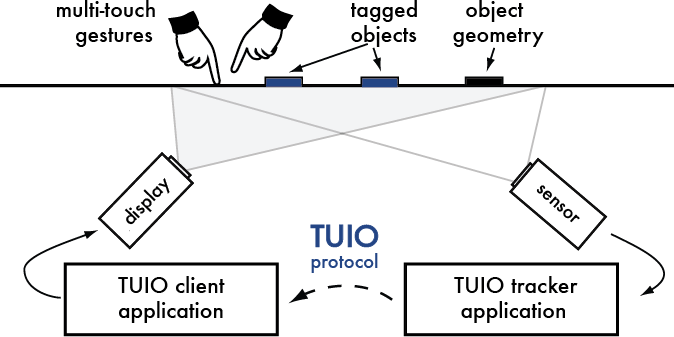
\includegraphics[width=15cm]{figures/TUIO_platform_diagram.png}
\end{center}
	\caption{Diagram of the TUIO protocol}
	\label{fig:TUIO_platform_diagram}
\end{figure}


%\signature

\end{document}